\vspace{-3cm}\chapter{题目3. 接口的威力}

\section{3.1 题目}

\subsection{3.1.1 任务一}
题目2中的图形类型的行为能力都是从绘制角度考虑的,但是一个图形类型除了具有被绘制的特点外,还有几何特征,比如面积。解决这个问题看似很简单:
为每个图形类型增加一个求解面积的成员方法就可以了。但是会发现:并不是所有能够绘制的图形都具有求解面积的行为,比如MyLine。那如何能够让应该具
有面积特征的图形有求解面积的行为,不具有面积特征的图形就不具有求解面积的行为,同时还不破坏它们具有可以被绘制的多态效果的现状呢?Java 的接口
类型可以助力完成上面的目标。本题第1个任务:请为该题目修改题目2中的图形类型,并绘制出新的图形类型之间的结构图。

扩展内容:再大胆一点…如何让 DrawPanel 类型可以绘制更多的东西(并不局限于图形类型的对象)?怎么修改
DrawPanel 中的数据成员类型以及构造方法?怎么定义类型使其能在 DrawPanel 上进行绘制?

\subsection{3.1.2 任务二}

依然尝试使用接口,比如创建了一个 MyTime 类型(这个类型第 1 个作业中被创建过),在 DrawPanel 上就可以绘制一个根据 MyTime 
对象中的数据所表现出来的一个时钟。(DrawPanel 原有的绘制其他图形的能力应该依然保持。)如下图所示:

\begin{figure}[H]
    \centering
    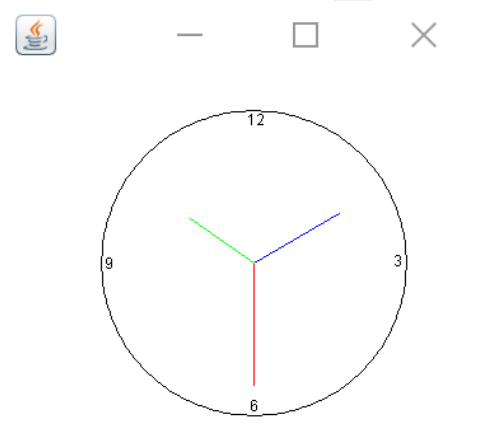
\includegraphics[width = 0.4\textwidth]{../pic/3/3.1.png}
\end{figure}

\section{3.2 题目分析}

本题任务一中的扩展内容我们已经在问题2中顺带解决,即创建一个 Drawable 接口,

\subsection{3.2.1 面积接口与实现}

对于可计算面积的图形也可以创建一个 calcAreable 接口以实现,接口内应定义返回面积的函数 double area(); 

在我们已定义的类中 MyRectangle 和 MyCircle 需要实现这一接口如下

\begin{figure}[H]
    \centering
    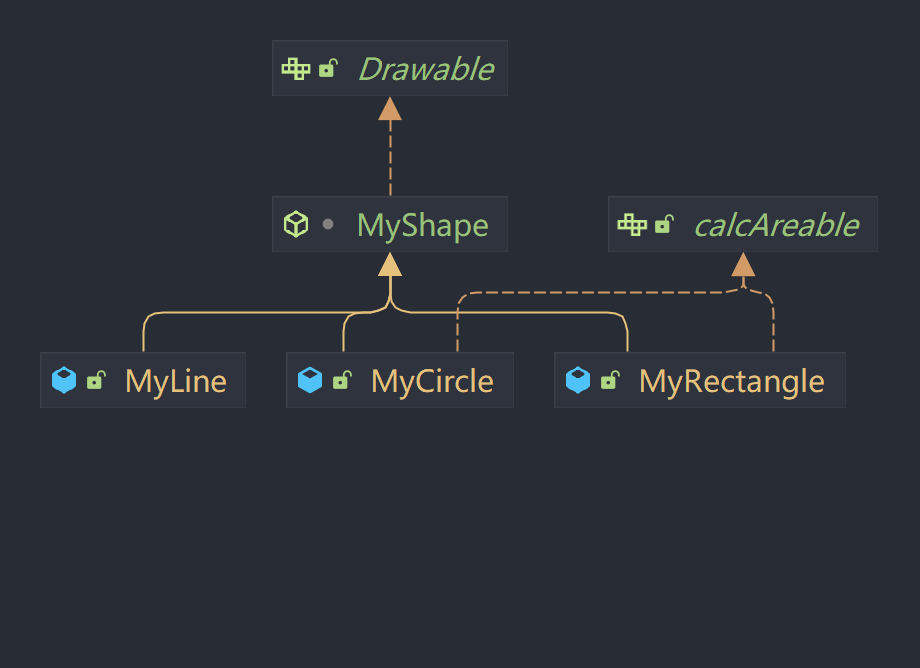
\includegraphics[width = 0.6\textwidth]{../pic/3/3.2.png}
\end{figure}


\begin{lstlisting}[language = Java]
public class MyRectangle extends MyShape implements calcAreable {
    // .....
    @Override
    public double area() {
		return (x_High - x_Low)*(y_High - y_Low);
	}
}
\end{lstlisting}

\begin{lstlisting}[language = Java]
public class MyCircle extends MyShape implements calcAreable {
    // .....
    @Override
	public double area() {
		return Math.pow(radix,2)*Math.PI;
	}
}
\end{lstlisting}

\subsection{3.2.2 绘制时钟}
 
多亏了提前看到第三题从而在第二题进行了二次抽象,依照已有的类和接口不难得出,我们只需将已经写好的 MyTime 类实现 Drawable 接口。
而根据题目,时钟的绘制分为三部分

\begin{enumerate}
    \item 绘制圆形外壳. 这一步只需在以窗口的中心为圆心画圆即可
    \item 标出四个时钟节点. 这一步需要用到 Graphics 的 drawString 方法,为使时钟更加美观,需要多次调整参数;
    \item 绘制三条直线. 这里为了方便我们绘制新建一个 MyLine 的构造方法,参考极坐标系下画直线的过程,如下
    \begin{lstlisting}[language = Java]
    public MyLine(int x, int y, int length, double rad, Color c) {
        this(x, y, x + (int) (length * Math.cos(rad)), y + (int) (length * Math.sin(rad)),c);
    }
    \end{lstlisting}
    随后经过数学计算即可得到每个指针对应的参数和其数值大小的关系,为了使模拟更加逼真,我在更高级的时间角度上加了更低角度的偏差。
    \item 为了便于展示,在时钟的上方再用 drawString 打印出时间.
\end{enumerate}

\section{3.3 运行结果展示}

时钟运行结果如下
\begin{figure}[H]
    \centering
    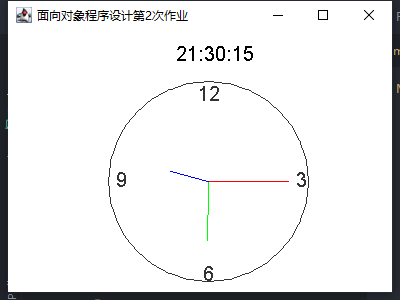
\includegraphics[width = 0.6\textwidth]{../pic/3/3.3.png}
\end{figure}

\section{3.4 主干代码展示}

\begin{lstlisting}[language = Java]
public class MyTime implements Drawable {
    // ....
    @Override
    public void draw(Graphics g) {
        final int CENTER_X = 200, CENTER_Y = 150, RADIX = 100, FONT_SIZE = 20;
        g.drawOval(CENTER_X - RADIX, CENTER_Y - RADIX, 2 * RADIX, 2 * RADIX);

        Font font = new Font("Arial", Font.PLAIN, FONT_SIZE);
        g.setFont(font);
        g.drawString("12", CENTER_X - FONT_SIZE / 2, CENTER_Y - RADIX + FONT_SIZE);
        g.drawString("3", CENTER_X + RADIX - FONT_SIZE / 2 - 2, CENTER_Y + FONT_SIZE / 3);
        g.drawString("6", CENTER_X - FONT_SIZE / 4, CENTER_Y + RADIX);
        g.drawString("9", CENTER_X - RADIX + FONT_SIZE / 2 - 2, CENTER_Y + FONT_SIZE / 3);

        double second_angle = (float) second / 30 * Math.PI;
        MyLine second_line = new MyLine(CENTER_X, CENTER_Y, 80, second_angle - Math.PI / 2, Color.red);
        second_line.draw(g);

        double minute_angle = (float) minute/ 30 * Math.PI + second_angle / 60;
        MyLine minute_line = new MyLine(CENTER_X, CENTER_Y, 60, minute_angle - Math.PI / 2, Color.green);
        minute_line.draw(g);

        double hour_angle = (float)hour/6 *Math.PI + minute_angle / 12;
        MyLine hour_line = new MyLine(CENTER_X, CENTER_Y, 40, hour_angle - Math.PI / 2, Color.blue);
        hour_line.draw(g);

        g.setColor(Color.black);
        g.drawString(this.toUniversalString(),CENTER_X - RADIX/2, CENTER_Y - RADIX - FONT_SIZE );
    }
}
\end{lstlisting}

\section{3.5 总结和收获}

在理解和掌握了接口的用法和思想后,不难发现本题的大体框架其实很简单,复杂的是本题中具体处理上的细节,
包括 Font 类的创建,drawString的参数,时钟怎么绘制更好看等等。


% 1、题目
% 2、数据设计
% 3、算法设计
% 4、主干代码说明
% 5、运行结果展示
% 6、总结和收获